\documentclass[tikz,border=2pt]{standalone}
\usepackage{amsmath,amssymb}
\usepackage{pgfplots}
\pgfplotsset{compat=1.18}
\usetikzlibrary{arrows.meta}
\begin{document}
% One path of S(t) with claim rate 2 per year and fixed severity 100 (illustrative arrival times
% 0.35, 0.8, 1.1, 1.75): constant between arrivals, jumps of 100 at arrivals; mean E[S(t)] = 200t.
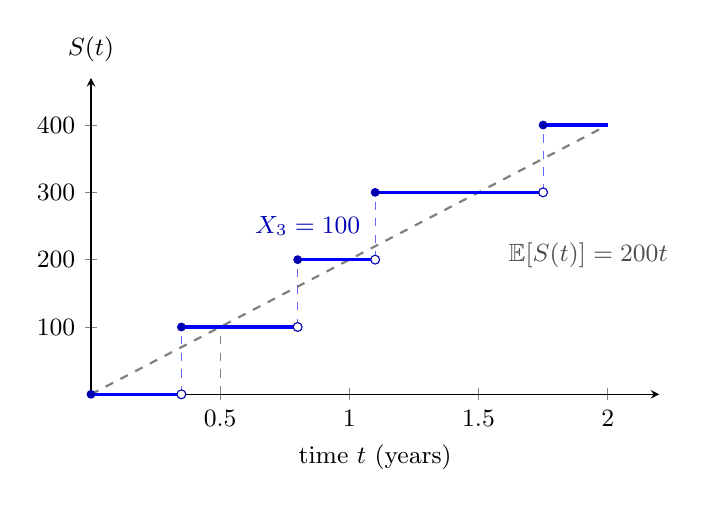
\begin{tikzpicture}[font=\small, >={Latex[length=2mm]}]
  \begin{axis}[
    axis lines=left, xmin=0, xmax=2.2, ymin=0, ymax=470,
    xtick={0.5,1,1.5,2}, ytick={100,200,300,400},
    xlabel={time $t$ (years)}, ylabel={$S(t)$},
    ylabel style={rotate=-90, anchor=south, at={(axis description cs:0,1.02)}},
    width=8.8cm, height=5.6cm, clip=false]
    \draw[gray, thick, dashed] (axis cs:0,0) -- (axis cs:2,400);
    \node[gray!60!black, anchor=north west] at (axis cs:1.58,240) {$\mathbb E[S(t)]=200t$};
    \draw[gray, thin, dashed] (axis cs:0.5,0) -- (axis cs:0.5,100);
    % path: horizontal pieces, closed dot at the left end, open dot at the right end
    \draw[blue, very thick] (axis cs:0,0) -- (axis cs:0.35,0);
    \draw[blue, very thick] (axis cs:0.35,100) -- (axis cs:0.8,100);
    \draw[blue, very thick] (axis cs:0.8,200) -- (axis cs:1.1,200);
    \draw[blue, very thick] (axis cs:1.1,300) -- (axis cs:1.75,300);
    \draw[blue, very thick] (axis cs:1.75,400) -- (axis cs:2,400);
    \draw[blue!60, thin, dashed] (axis cs:0.35,0) -- (axis cs:0.35,100);
    \draw[blue!70!black, fill=white] (axis cs:0.35,0) circle (1.6pt);
    \fill[blue!70!black] (axis cs:0.35,100) circle (1.6pt);
    \draw[blue!60, thin, dashed] (axis cs:0.8,100) -- (axis cs:0.8,200);
    \draw[blue!70!black, fill=white] (axis cs:0.8,100) circle (1.6pt);
    \fill[blue!70!black] (axis cs:0.8,200) circle (1.6pt);
    \draw[blue!60, thin, dashed] (axis cs:1.1,200) -- (axis cs:1.1,300);
    \draw[blue!70!black, fill=white] (axis cs:1.1,200) circle (1.6pt);
    \fill[blue!70!black] (axis cs:1.1,300) circle (1.6pt);
    \draw[blue!60, thin, dashed] (axis cs:1.75,300) -- (axis cs:1.75,400);
    \draw[blue!70!black, fill=white] (axis cs:1.75,300) circle (1.6pt);
    \fill[blue!70!black] (axis cs:1.75,400) circle (1.6pt);
    \fill[blue!70!black] (axis cs:0,0) circle (1.6pt);
    \node[blue!70!black, anchor=east] at (axis cs:1.08,250) {$X_3=100$};
  \end{axis}
\end{tikzpicture}
\end{document}
